\subsection{Projected Gamma}
\label{method:pg}
The projected gamma distribution, developed in \cite{nunez2019}, is built upon
  the product of $d$ independent gamma distributions.  That is, for
  ${\bf y} = (y_1,\ldots,y_d)^t$, and $y_i\sim\text{Ga}(\alpha_i,\beta_i)$, we
  define our starting point:
\begin{equation}
    f({\bf y}\mid{\bf \alpha},{\bf \beta}) = \prod_{j = 1}^d\text{Ga}(y_j\mid\alpha_j,\beta_j),
\end{equation}
where $\beta$ is specified as a rate parameter.  From that, we transform to
  $d$-dimensional spherical coordinates ${\bf y} \rightarrow (r,{\bf \theta})$
  as
\begin{equation}
  \label{eqn:transform}
  \begin{aligned}
    y_1     &= r\cos\theta_1,\\
    y_2     &= r\sin\theta_1\cos\theta_2\\
            &\vdots\\
    y_{d-1} &= r\sin\theta_1\ldots\sin\theta_{d-2}\\
    y_{d}   &= r\sin\theta_1\ldots\sin\theta_{d-1}
  \end{aligned}
\end{equation}
where $r = \lVert {\bf y}\rVert_{2}$, the euclidean norm of ${\bf y}$.  The
  inverse of this transformation is:
\begin{equation}
  \label{eqn:invtransform}
  \begin{aligned}
    \theta_1     &= \cos^{-1}\left[\frac{y_1}{\lVert y_{1:d}\rVert_2}\right]\\
    \theta_2     &= \cos^{-1}\left[\frac{y_2}{\lVert y_{2:d}\rVert_2}\right]\\
                 &\vdots\\
    \theta_{d-1} &= \cos^{-1}\left[\frac{y_{d-1}}{\lVert y_{(d-1):d}\rVert_2}\right].
  \end{aligned}
\end{equation}
The Jacobian of this transformation is
\begin{equation*}
r^{d-1}\prod_{i = 1}^{d-2}(\sin\theta_i)^{d-1-i}.
\end{equation*}
This creates the distribution over $r,{\bf \theta}$.  The full conditional for
  $r$ takes the form of a Gamma random variable, and we can integrate it out as
  such.  This leaves the \emph{projected gamma distribution},
\begin{equation}
    \text{PG}({\bf \theta}\mid{\bf \alpha},{\bf \beta}) = \frac{\Gamma(A)\beta_d^{\alpha_d}}{B^A\Gamma(a_d}\left(\prod_{j = 1}^{d-1}\frac{\beta_j^{\alpha_j}}{\Gamma(\alpha_j)}(\cos\theta_j)^{\alpha_j - 1}(\sin\theta_j)^{(\sum_{h = j + 1}^d\alpha_h) - 1}\right)\mathcal{I}_{(0,\pi/2)^{d-1}}({\bf \theta})
\end{equation}
where
\begin{equation}
    A = \sum_{j = 1}^d\alpha_j \hspace{1cm}\text{and}\hspace{1cm}B = \beta_1\cos\theta_1 + \sum_{j = 2}^{d-1}\left(\beta_j\cos\theta_j\prod_{i = 1}^{j-1}\sin\theta_i\right) + \beta_d\prod_{j = 1}^d-1\sin\theta_j.
\end{equation}
As is, this model is not identifiable, as taking
  ${\bf \beta}^{(2)} = \alpha {\bf \beta}^{(1)}$ will still yield the same
  distribution of angles. Following \cite{nunez2019}, we have opted to place a
  restriction on $\beta$ such that $\beta_1 := 1$, thus
  ${\bf \beta} = (1, \beta_2, \ldots, \beta_d)^t$.

Inference on this model can take two forms: ${\bf \alpha}$ and ${\bf \beta}$ in
  this form can not be broken down into known-form full conditionals, so we can
  conduct a Metropolis Hastings step for every component, or do a joint proposal
  Metropolis Hastings step for all components at once.  Alternatively, using
  $f(r,{\bf \theta})$, we recognize that $\alpha_i\mid r$ is independent of
  $\alpha_j\mid r$, so we can sample the latent $r$ and conduct independent
  Gibbs steps for each component.  Further, in sampling the $\alpha_j$'s, we can
  integrate out $\beta_j$. Within the Gibbs sampler, we sample $r$, then each
  $\alpha_j\mid r$, then each $\beta_j\mid r, \alpha_j$.  This leads to fast
  convergence, with the only Metropolis Hastings step being for the
  $\alpha_j$'s.  Both $r$ and the $\beta_j$'s are Gamma distributed.

For simplicity, let ${\bf y^{\prime}} = r^{-1}{\bf y}$.  That is,
  ${\bf y^{\prime}}$ is a function of the angular data--from~\eqref{eqn:transform},
  ${\bf y^{\prime}} = {\bf y}/r$, the projection of the ${\bf y}$ vector onto
  the unit hypersphere. We generate a latent $r$, and their product is the
  latent ${\bf y}$.  Given ${\bf y}$, the posterior distributions for
  $(\alpha_i, \beta_i)$, $(\alpha_j,\beta_j)$, $i\neq j$ are independent.

As~\cite{nunez2019} shows, the projected gamma distribution is a flexible model
  for representing data on the positive orthant of the unit hypersphere.  As such,
  given our application restricts us to this domain, one can see that this might be a
  natural choice of distribution for our purpose.

\begin{figure}[h]
  \centering
  \label{fig:vanillamix}
  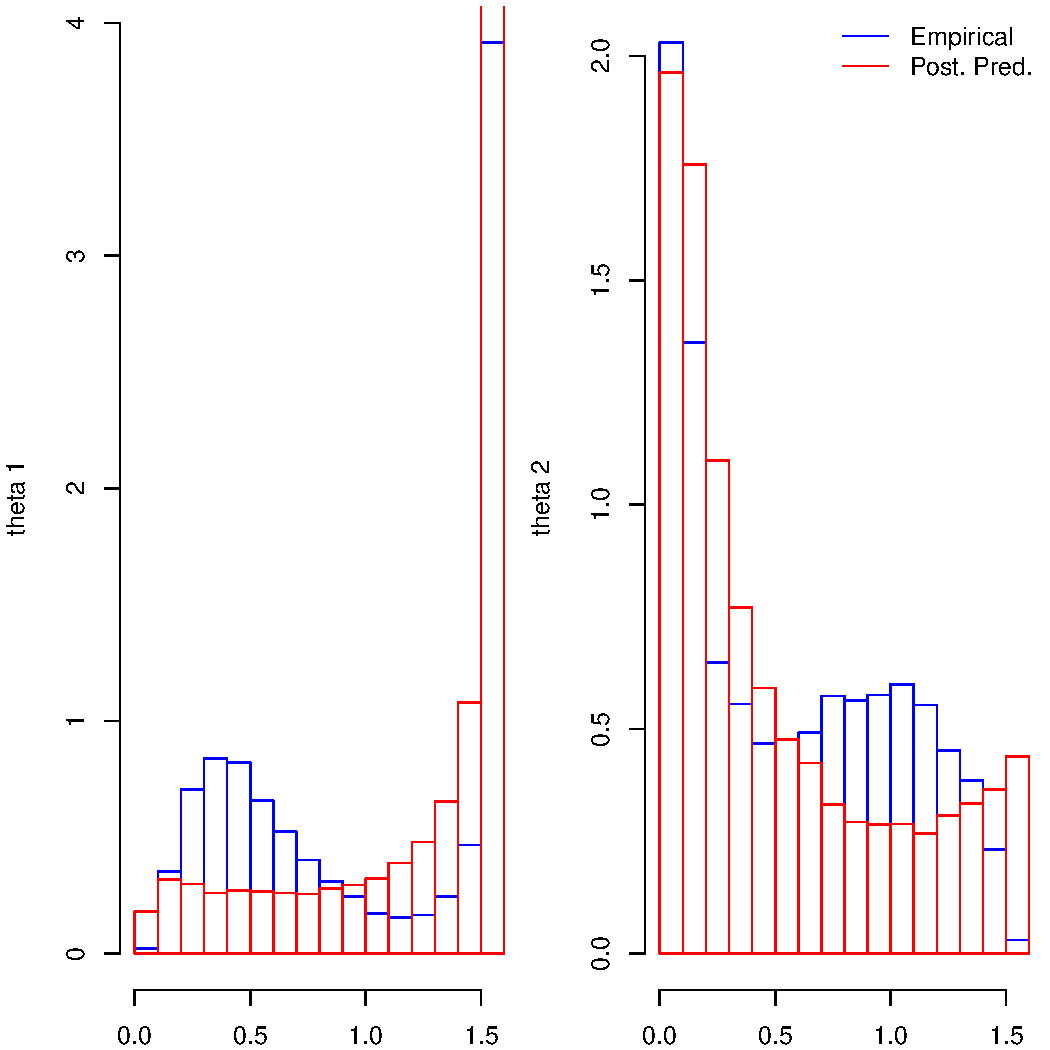
\includegraphics{./images/justification}
  \caption{Histograms of Empirical vs Posterior-predictive angular data originating
            from a simulated 3-dimensional gamma dataset.}
\end{figure}

However, as flexible as it is, it alone is not sufficient for our purpose.  Supposing
  a given dataset is the result of two or more generating distributions, then using a
  a single distribution to represent this dataset becomes untenable.  In Figure~\ref{fig:vanillamix}
  we see the empirical distribution a 2-component mixture of projected gammas, plotted
  against the posterior predictive distribution of a projected gamma model fitted to
  that dataset.  As we can see, it has trouble representing the nuances of the two
  component mixture.


% EOF
